% SkillLens final report: Springer LNCS skeleton.
% Compile on Overleaf: create a project from Springer's "LNCS" template (it provides llncs.cls and
% splncs04.bst), then upload this folder (main.tex, references.bib, architecture.tex, pseudocode.tex,
% figures/, tables/). Check the exact template version and any page limit in the course guideline.
%
% Everything inside \yaz{...} is a prompt for YOUR text. Replace it with your own words and delete
% the prompt. Numbers in tables/figures come from results/ and checkpoints/ (scripts/make_figures.py).
\documentclass[runningheads]{llncs}
\usepackage[T1]{fontenc}
\usepackage[utf8]{inputenc}
\usepackage{graphicx}
\usepackage{booktabs}
\usepackage{amsmath}
\usepackage{xcolor}
\usepackage{algorithm}
\usepackage{algpseudocode}
\usepackage{tikz}
\usetikzlibrary{positioning,arrows.meta,fit,backgrounds}
\usepackage{hyperref}

\newcommand{\yaz}[1]{\textcolor{red}{\textbf{[YAZ:} #1\textbf{]}}}

\begin{document}

\title{SkillLens: Deep Learning-Based Developer Skill Assessment and Job Matching}
\titlerunning{SkillLens}
\author{\yaz{Adın Soyadın}}
\authorrunning{\yaz{Ad Soyad}}
\institute{\yaz{Bölüm, Üniversite, e-posta}}
\maketitle

\begin{abstract}
\yaz{150--250 kelime. Problem ne? Hangi veri (SkillSpan)? Hangi iki model? Uygulama ne yapıyor (CV, quiz,
eşleştirme, yol haritası)? Ölçülen temel sonuç ne: test F1 ve gecikme (Tablo~\ref{tab:scores},
Tablo~\ref{tab:eff})? Bir cümlelik sonuç.}
\keywords{Skill extraction \and Sequence labelling \and BiLSTM \and DistilBERT \and Job matching}
\end{abstract}

% =====================================================================
\section{Introduction}
\yaz{İş ilanlarındaki beceri gereksinimlerini otomatik anlamak neden zor? (uzun ve belirsiz ifadeler,
yumuşak beceriler, aynı becerinin farklı yazımları) Öğrenciler/adaylar için neden önemli?}

\yaz{Araştırma sorunu açıkça yaz: BiLSTM ile fine-tune edilmiş DistilBERT aynı veride beceri ve bilgi
ifadelerini ne kadar doğru ve ne kadar hızlı çıkarıyor?}

\yaz{Raporun geri kalanının kısa planı.}

% =====================================================================
\section{Contribution}
\yaz{Madde madde, kendi yaptıkların: (1) iki modeli aynı veri, aynı görev temsili (iki etiket başlığı)
ve aynı değerlendirme ile kıyaslama; (2) çıkarılan gereksinimleri CV beyanı ve quiz kanıtıyla ayrı
ayrı eşleştiren açıklanabilir skor; (3) ön koşullu yol haritası ve kurs önerisi; (4) FastAPI + web
prototipi. Her maddenin neden değerli olduğunu bir cümleyle açıkla.}

% =====================================================================
\section{Similar Studies}
\yaz{SkillSpan veri seti ve makalesi \cite{zhang2022skillspan}: ne öneriyor, Skill/Knowledge ayrımını
nasıl tanımlıyor, sen nasıl kullandın?}

\yaz{BiLSTM ile dizi etiketleme \cite{hochreiter1997lstm,graves2005bilstm,huang2015bilstmcrf,lample2016ner}:
neden güçlü bir temel model? Senin modelinde CRF yok, bunu belirt.}

\yaz{Transformer tabanlı modeller \cite{devlin2019bert,sanh2019distilbert}: DistilBERT'i neden seçtin
(boyut/hız)? Hugging Face Transformers \cite{wolf2020transformers} kullandığını yaz.}

\yaz{BIO gösterimi ve varlık düzeyinde değerlendirme \cite{ramshaw1995chunking,tjongkimsang2003conll}.}

% =====================================================================
\section{Methodology}
\yaz{Bir paragraf: sistemin girişten çıkışa genel akışı (Şekil~\ref{fig:arch}).}

\begin{figure}[t]
\centering
\resizebox{\textwidth}{!}{% System architecture (TikZ). Needs \usepackage{tikz} and \usetikzlibrary{positioning,arrows.meta,fit,backgrounds}.
% Nodes sit on fixed coordinates (cm) so nothing overlaps when the figure is scaled.
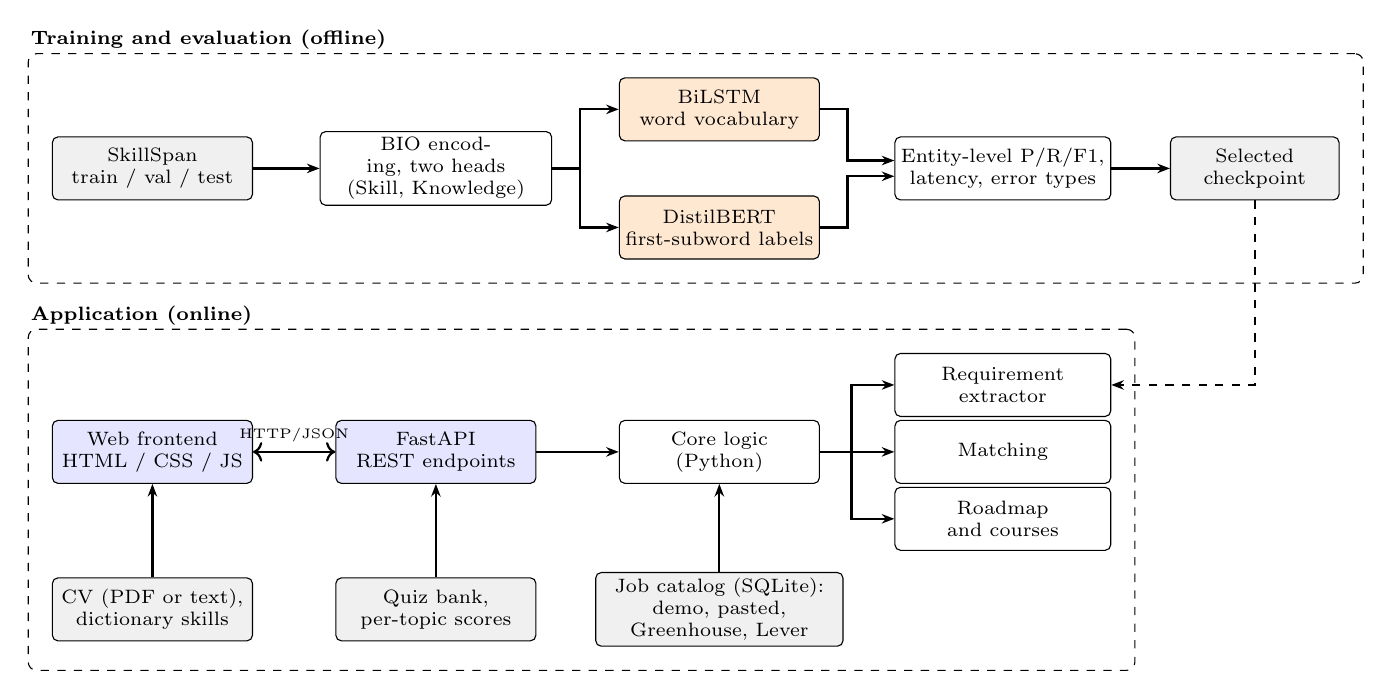
\begin{tikzpicture}[
  font=\scriptsize,
  box/.style={draw, rounded corners=2pt, align=center, minimum height=8mm, text width=#1, inner sep=2pt, fill=white},
  box/.default=24mm,
  data/.style={box=#1, fill=gray!12}, data/.default=24mm,
  model/.style={box=#1, fill=orange!18}, model/.default=24mm,
  app/.style={box=#1, fill=blue!10}, app/.default=24mm,
  arr/.style={-{Stealth[length=1.6mm]}, thick},
  group/.style={draw, dashed, rounded corners=3pt, inner sep=3mm},
  lbl/.style={font=\scriptsize\bfseries, anchor=south west, inner sep=1pt}
]
% ---------------- training and evaluation (offline)
\node[data]          (ss)   at (0, 0)      {SkillSpan\\train / val / test};
\node[box=28mm]      (prep) at (3.6, 0)    {BIO encoding, two heads\\(Skill, Knowledge)};
\node[model]         (lstm) at (7.2, 0.75) {BiLSTM\\word vocabulary};
\node[model]         (bert) at (7.2, -0.75) {DistilBERT\\first-subword labels};
\node[box=26mm]      (eval) at (10.8, 0)   {Entity-level P/R/F1,\\latency, error types};
\node[data=20mm]     (ckpt) at (14.0, 0)   {Selected\\checkpoint};
\draw[arr] (ss) -- (prep);
\draw[arr] (prep.east) -- ++(0.35,0) |- (lstm.west);
\draw[arr] (prep.east) -- ++(0.35,0) |- (bert.west);
\draw[arr] (lstm.east) -- ++(0.35,0) |- ([yshift=1mm]eval.west);
\draw[arr] (bert.east) -- ++(0.35,0) |- ([yshift=-1mm]eval.west);
\draw[arr] (eval) -- (ckpt);
\begin{scope}[on background layer]
  \node[group, fit=(ss)(lstm)(bert)(ckpt)] (train) {};
\end{scope}
\node[lbl] at (train.north west) {Training and evaluation (offline)};

% ---------------- application (online)
\node[app]           (web)   at (0, -3.6)   {Web frontend\\HTML / CSS / JS};
\node[app]           (api)   at (3.6, -3.6) {FastAPI\\REST endpoints};
\node[box]           (core)  at (7.2, -3.6) {Core logic\\(Python)};
\node[box=26mm]      (ext)   at (10.8, -2.75) {Requirement extractor};
\node[box=26mm]      (match) at (10.8, -3.6)  {Matching};
\node[box=26mm]      (road)  at (10.8, -4.45) {Roadmap and courses};
\node[data]          (cv)    at (0, -5.6)   {CV (PDF or text),\\dictionary skills};
\node[data]          (quiz)  at (3.6, -5.6) {Quiz bank,\\per-topic scores};
\node[data=30mm]     (jobs)  at (7.2, -5.6) {Job catalog (SQLite):\\demo, pasted, Greenhouse, Lever};
\draw[arr, <->] (web) -- node[above, font=\tiny] {HTTP/JSON} (api);
\draw[arr] (api) -- (core);
\draw[arr] (core.east) -- ++(0.4,0) |- (ext.west);
\draw[arr] (core) -- (match);
\draw[arr] (core.east) -- ++(0.4,0) |- (road.west);
\draw[arr] (cv) -- (web);
\draw[arr] (quiz) -- (api);
\draw[arr] (jobs) -- (core);
\draw[arr, dashed] (ckpt.south) |- (ext.east);
\begin{scope}[on background layer]
  \node[group, fit=(web)(cv)(jobs)(ext)(road)] (appg) {};
\end{scope}
\node[lbl] at (appg.north west) {Application (online)};
\end{tikzpicture}
}
\caption{SkillLens architecture: offline training and evaluation of both taggers (top) and the
online application (bottom). The selected checkpoint is used by the requirement extractor.}
\label{fig:arch}
\end{figure}

\subsection{Data}
\yaz{SkillSpan'i nereden aldın, hangi split'leri kullandın, etiketler nasıl (Tablo~\ref{tab:data})?
Skill ve Knowledge'ın ayrı BIO dizileri olduğunu ve örtüşmeyi (train'de 97 cümle) neden iki başlıkla
temsil ettiğini açıkla. Lisans: Hugging Face kartı CC BY 4.0; makaleye göre TECH ilanları CC BY-SA
(bkz. docs/data\_notes.md).}

\begin{table}[t]
\centering
\caption{SkillSpan splits used in this work (sentences and span counts, measured by
\texttt{scripts/inspect\_skillspan.py}). Overlap = sentences where a token is inside both a Skill
and a Knowledge span.}
\label{tab:data}
\begin{tabular}{lrrrrr}
\toprule
Split & Sentences & Skill spans (B) & Knowledge spans (B) & Overlap sent. & Max length \\
\midrule
Train & 4800 & 2221 & 2969 & 97 & 748 \\
Validation & 3174 & 1070 & 1093 & 25 & 80 \\
Test & 3569 & 1090 & 1174 & 12 & 149 \\
\bottomrule
\end{tabular}
\end{table}

\subsection{Models}
\yaz{BiLSTM: gömme $\rightarrow$ 2 katmanlı çift yönlü LSTM $\rightarrow$ iki sınıflandırıcı; sözlük yalnız
train'den, \texttt{<unk>}, padding maskesi, packed sequence. DistilBERT: ilk alt-kelime etiketleme,
özel token'lar ve diğer alt-kelimeler loss dışında, uzun cümleler için pencere. Loss = iki başlığın
toplamı. Ayarlar Tablo~\ref{tab:hparams}'te.}

\begin{table}[t]
\centering
\caption{Training settings (from \texttt{run\_info.json} of each run). Both use seed 42 and keep the
epoch with the best validation F1.}
\label{tab:hparams}
\resizebox{\textwidth}{!}{%
\begin{tabular}{lll}
\toprule
 & BiLSTM & DistilBERT \\
\midrule
Encoder & embedding 100, BiLSTM $2\times128$ & \texttt{distilbert-base-cased} \\
Heads & 2 linear (Skill, Knowledge), O/B/I & 2 linear (Skill, Knowledge), O/B/I \\
Optimiser & Adam, lr $10^{-3}$, clip 5 & AdamW, lr $5\cdot10^{-5}$, wd 0.01, warm-up 10\%, clip 1 \\
Batch / dropout & 32 / 0.3 & 16 / 0.1 \\
Max. epochs / patience & 30 / 5 & 10 / 3 \\
Other & vocab from train, min freq.\ 2 & fp16; train windows 256, inference 512 subwords \\
\bottomrule
\end{tabular}}
\end{table}

\subsection{Evaluation protocol}
\yaz{Varlık düzeyinde P/R/F1: tahmin ancak cümle, başlangıç, bitiş ve tür aynıysa doğru. Kendi metrik
kodunu seqeval \cite{nakayama2018seqeval} ile test ettiğini yaz. Gecikme: aynı GPU, batch 1, 500 test
cümlesi, 20 ısınma, ön işleme dahil, medyan/p90. Hata türleri: FP, FN, sınır hatası. Test setine
yalnız son ölçümde dokunulduğunu belirt.}

\subsection{Application: CV, quiz, matching and roadmap}
\yaz{CV becerileri neden ilan modeliyle değil sözlükle çıkarılıyor ve kullanıcı onaylıyor? Quiz (5 konu,
65 soru, şıklar her oturumda karıştırılıyor, cevaplar teslimden önce gönderilmiyor). Skor formülleri
(Algoritma~\ref{alg:match}), yol haritası (Algoritma~\ref{alg:roadmap}), ilan kaynakları (demo,
yapıştırılan, Greenhouse/Lever). Gereksinim çıkarma: Algoritma~\ref{alg:extract}.}

% Pseudocode drafts derived from the implementation (core/extractor.py, core/matching.py, core/roadmap.py).
% Needs \usepackage{algorithm} and \usepackage{algpseudocode}. Check each step against the code before submitting.

\begin{algorithm}[t]
\caption{Requirement extraction from a job ad}\label{alg:extract}
\begin{algorithmic}[1]
\Require job text $T$, trained tagger $M$ with heads $H=\{\textsc{Skill},\textsc{Knowledge}\}$, skill dictionary $D$
\Ensure requirements $R$ (phrase, type, character offsets, canonical skills)
\State $S \gets$ \Call{SplitSentences}{$T$} \Comment{periods, bullets, line breaks}
\For{each sentence $s \in S$}
  \State $w \gets$ \Call{Tokenize}{$s$} \Comment{keeps C\#, C++, Node.js; stores offsets}
  \For{each head $h \in H$}
    \State $y_h \gets M_h(w)$ \Comment{O/B/I per word}
    \For{each span $(a,b) \in$ \Call{BIOtoSpans}{$y_h$}}
      \State trim punctuation at the span edges
      \State add $(T[\mathit{off}(a):\mathit{off}(b)], h, \text{offsets}, D.\textsc{Normalize}(\cdot))$ to $R$
    \EndFor
  \EndFor
\EndFor
\State for spans with no canonical skill: map to the skill of the most similar alias (Sentence-BERT) if cosine $\ge 0.75$
\State add dictionary hits of $D$ in $T$ not covered by any model span, flagged as \emph{dictionary}
\State merge repeated mentions with the same type and canonical skills
\State \Return $R$, its canonical skill set, and the phrases with no canonical skill (kept visible)
\end{algorithmic}
\end{algorithm}

\begin{algorithm}[t]
\caption{Explainable job match}\label{alg:match}
\begin{algorithmic}[1]
\Require job skills $J$, confirmed CV skills $C$, quiz results $Q[\mathit{topic}] = (\mathit{correct}, \mathit{total})$
\Ensure per-skill status and scores
\If{$J = \emptyset$} \State \Return ``could not be calculated'' \EndIf
\For{each $j \in J$}
  \State $t \gets$ quiz topic of $j$ (may be none)
  \If{$t \in Q$ and $Q[t].\mathit{ratio} < 0.6$} \State status $\gets$ weak quiz
  \ElsIf{$j \in C$ and $t \in Q$} \State status $\gets$ CV + quiz
  \ElsIf{$t \in Q$} \State status $\gets$ quiz only
  \ElsIf{$j \in C$} \State status $\gets$ CV only
  \Else \State status $\gets$ missing
  \EndIf
\EndFor
\State $\mathit{cvCov} \gets |J \cap C| / |J|$
\State $T_J \gets$ quiz topics of $J$; \quad $T_m \gets T_J \cap \mathrm{keys}(Q)$
\State $\mathit{quizPerf} \gets \mathrm{mean}_{t \in T_m} Q[t].\mathit{ratio}$; \quad $\mathit{quizCov} \gets |T_m| / |T_J|$
\If{$T_m = \emptyset$} \State $\mathit{combined} \gets \mathit{cvCov}$ \Comment{stated to the user}
\Else \State $\mathit{combined} \gets 0.5\,\mathit{cvCov} + 0.5\,\mathit{quizPerf}$
\EndIf
\State \Return statuses, $\mathit{cvCov}$, $\mathit{quizPerf}$, $\mathit{quizCov}$, $\mathit{combined}$
\end{algorithmic}
\end{algorithm}

\begin{algorithm}[t]
\caption{Learning roadmap with prerequisites}\label{alg:roadmap}
\begin{algorithmic}[1]
\Require match result, user evidence $E$ (CV skills and topics passed in the quiz), topic graph $G$ (skills, prerequisites, goal)
\Ensure ordered steps
\State $\mathit{gaps} \gets$ skills with status weak quiz (first), then missing
\State $\mathit{steps} \gets [\,]$, $\mathit{placed} \gets \emptyset$
\Procedure{Add}{$v$, reason}
  \If{$v \in \mathit{placed}$} \State merge reason into the existing step; \Return \EndIf
  \For{each prerequisite $p$ of $v$ in $G$}
    \If{no skill of $p$ is in $E$} \State \Call{Add}{$p$, ``prerequisite for $v$''} \EndIf
  \EndFor
  \State append $(v, \text{reason}, \text{goal}(v), \text{courses}(v))$ to $\mathit{steps}$; $\mathit{placed} \gets \mathit{placed} \cup \{v\}$
\EndProcedure
\For{each skill $g \in \mathit{gaps}$}
  \If{$g$ is taught by a topic $v \in G$} \State \Call{Add}{$v$, why $g$ is a gap}
  \Else \State append a generic step for $g$
  \EndIf
\EndFor
\State \Return $\mathit{steps}$ \Comment{$G$ is checked to be acyclic when loaded}
\end{algorithmic}
\end{algorithm}


% =====================================================================
\section{Results}

\begin{table}[t]
\centering
\caption{Entity-level precision, recall and F1 on the SkillSpan test split (3,569 sentences).}
\label{tab:scores}
\resizebox{\textwidth}{!}{\begin{tabular}{l ccc ccc ccc}
\hline
 & \multicolumn{3}{c}{Overall} & \multicolumn{3}{c}{Skill} & \multicolumn{3}{c}{Knowledge} \\
Model & P & R & F1 & P & R & F1 & P & R & F1 \\
\hline
BiLSTM & 0.407 & 0.394 & 0.400 & 0.291 & 0.260 & 0.275 & 0.499 & 0.518 & 0.508 \\
DistilBERT & 0.512 & 0.548 & 0.530 & 0.420 & 0.439 & 0.429 & 0.594 & 0.650 & 0.621 \\
\hline
\end{tabular}
}
\end{table}

\begin{table}[t]
\centering
\caption{Model size, selected epoch and inference latency per sentence (batch size 1, 500 test
sentences after 20 warm-up runs, including tokenisation and decoding; RTX 3050 Ti Laptop GPU).}
\label{tab:eff}
\begin{tabular}{l r c r r r}
\hline
Model & Params & Best val. epoch & Median ms & p90 ms & Mean ms \\
\hline
BiLSTM & 1.1M & 22 & 2.21 & 4.40 & 2.68 \\
DistilBERT & 65.2M & 7 & 6.20 & 7.97 & 6.54 \\
\hline
\end{tabular}

\end{table}

\begin{table}[t]
\centering
\caption{Test scores over three training seeds (42, 13, 7): mean $\pm$ standard deviation. Each seed
selects its own checkpoint on validation F1. Produced by \texttt{scripts/aggregate\_seeds.py}.}
\label{tab:seeds}
\begin{tabular}{l ccc cc}
\hline
Model & P & R & F1 & F1 skill & F1 knowledge \\
\hline
BiLSTM & 0.389 $\pm$ 0.015 & 0.402 $\pm$ 0.011 & 0.395 $\pm$ 0.006 & 0.275 $\pm$ 0.010 & 0.499 $\pm$ 0.008 \\
DistilBERT & 0.520 $\pm$ 0.007 & 0.558 $\pm$ 0.009 & 0.538 $\pm$ 0.008 & 0.438 $\pm$ 0.008 & 0.627 $\pm$ 0.007 \\
\hline
\end{tabular}

\end{table}

\yaz{Tablo~\ref{tab:seeds}: sonuçlar seed'den seed'e ne kadar oynuyor? İki model arasındaki fark
(yaklaşık 0.14 F1) bu oynamaya (yaklaşık $\pm$0.01) göre büyük mü? Bu, farkın şans olmadığını mı gösteriyor?}

\begin{figure}[t]
\centering
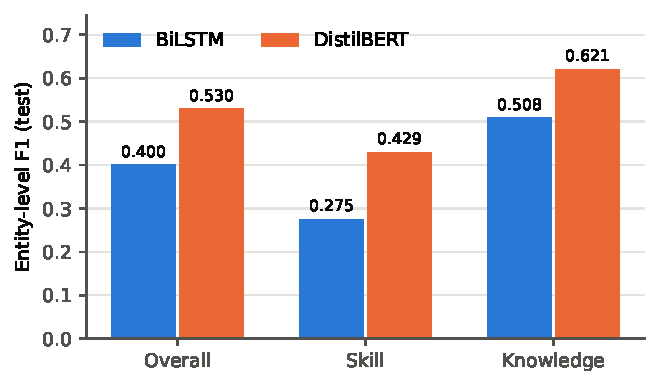
\includegraphics[width=0.49\textwidth]{figures/test_f1.pdf}\hfill
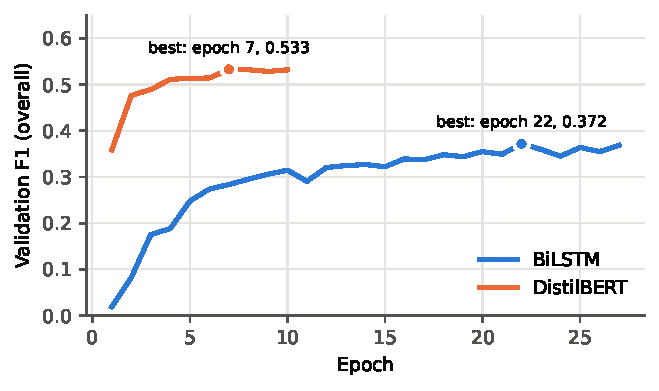
\includegraphics[width=0.49\textwidth]{figures/val_f1_curves.pdf}
\caption{Left: test F1 by span type. Right: validation F1 per epoch; dots mark the selected checkpoints.}
\label{fig:f1}
\end{figure}

\begin{figure}[t]
\centering
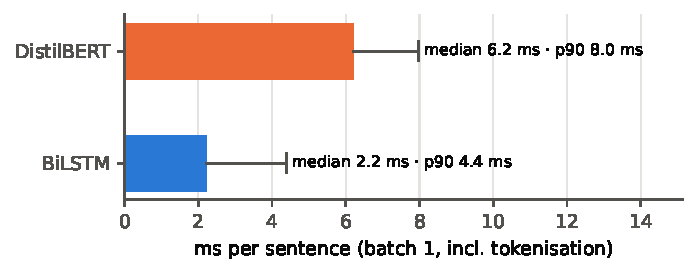
\includegraphics[width=0.49\textwidth]{figures/latency.pdf}\hfill
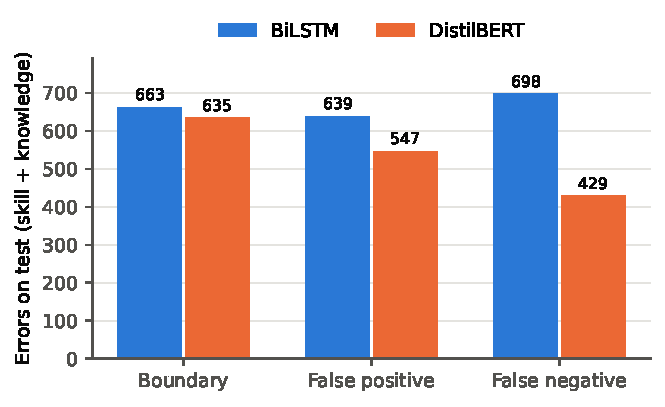
\includegraphics[width=0.49\textwidth]{figures/error_types.pdf}
\caption{Left: latency (bar = median, whisker = p90). Right: error types on the test split.}
\label{fig:lat}
\end{figure}

\yaz{Tablo~\ref{tab:scores} ve Şekil~\ref{fig:f1}'i kendi cümlelerinle yorumla: hangi model hangi türde
ne kadar iyi? Skill neden Knowledge'tan zor?}

\yaz{Hız (Tablo~\ref{tab:eff}, Şekil~\ref{fig:lat}): fark ne kadar ve uygulama için anlamı ne?
Uygulamada hangi modeli seçtin ve neden (validation sonucu + hız ihtiyacı)?}

\yaz{Hata analizi (Tablo~\ref{tab:errors}, Şekil~\ref{fig:lat} sağ): hangi hata türü baskın? Örneklerden
ne öğreniyoruz (sınırın kayması, genel ifadeler, noktalama)?}

\begin{table}[t]
\centering
\caption{Real DistilBERT errors from the test split (\texttt{results/errors\_distilbert.jsonl}).}
\label{tab:errors}
\resizebox{\textwidth}{!}{\begin{tabular}{l l p{2.3cm} p{2.3cm} p{5.2cm}}
\hline
Error & Type & Gold span & Predicted span & Sentence \\
\hline
False positive & skill & -- & dynamic & \footnotesize dynamic and experienced team - we are shapers and makers \\
False positive & skill & -- & contribution to software systems & \footnotesize \textbullet{} Successful contribution to software systems \\
False negative & skill & developmental toolsets & -- & \footnotesize * \textbullet{} Working proficiency in developmental toolsets \\
False negative & skill & achieve organizational goals & -- & \footnotesize * Ability to work in large collaborative teams to achieve organizational goals \\
Boundary & skill & developing multithreaded scalable concurrent applications & developing multithreaded scalable concurrent applications . & \footnotesize * \textbullet{} Competent with developing multithreaded scalable concurrent applications . \\
Boundary & skill & Ensure on-going health and stability of pipelines across multiple environments & Ensure on-going health and stability of pipelines & \footnotesize Ensure on-going health and stability of pipelines across multiple environments \\
\hline
\end{tabular}
}
\end{table}

\yaz{Demo: brifteki senaryoyu anlat (CV: Python, Git; ilan: Python, SQL, Git; quiz: Python güçlü, SQL
zayıf). Uygulama ne gösterdi (Git CV kanıtıyla, SQL yol haritasında)? Bir ekran görüntüsü ekle.
Canlı ilan içe aktarmayı da yaz: Greenhouse panosundan 15 gerçek ilan alındı, tekrar içe aktarmada
15'i de ``değişmedi'' kaldı (22.11.2026'da denendi).}

% =====================================================================
\section{Conclusion}
\yaz{Araştırma sorusunun cevabı (sayılarla). Sınırlamalar: 3 seed (az), tek GPU, CRF yok, CV için sözlük
kapsamı, quiz bankası küçük, demo ilanlar sentetik, skor ağırlıkları sabit 0.5/0.5. Gelecek çalışma.}

\bibliographystyle{splncs04}
\bibliography{references}

\end{document}
